%\documentclass[12pt,handout]{beamer}
\documentclass{beamer}

\usepackage{pgfpages}
\usepackage{setspace}
\usepackage{tipa}
\usepackage{algorithmic}
\usepackage[font=scriptsize,labelformat=empty]{caption}
\usepackage[absolute,overlay]{textpos}

%\setbeameroption{show notes on second screen}
    %   OR
%\pgfpagesuselayout{8 on 1}[a4paper,border shrink=5mm]
%\setbeameroption{show notes}

\title[Speech Enhancement and Evaluation using Phoneme NMF]
{Speech Enhancement and Evaluation using Phoneme Non-negative Matrix Factorisation}
\author{Ashley~Gillman}
%\institute{James Cook University}
\institute[James Cook University \hspace{2em} \insertframenumber/\inserttotalframenumber]{James Cook University} % include slide no. in footer
\logo{\includegraphics[height=1cm]{fig/JCU_Logo&CampusStack_CMYK.eps}}

\usetheme{Szeged}
\usecolortheme{crane}
\setbeamertemplate{headline}{%
	\begin{beamercolorbox}[colsep=1.5pt]{upper separation line head}
	\end{beamercolorbox}
	\begin{beamercolorbox}{section in head/foot}
	    \vskip2pt\insertsectionnavigationhorizontal{\paperwidth}{}{\hfill}\vskip2pt
	\end{beamercolorbox}%
	\begin{beamercolorbox}[ht=10pt]{subsection in head/foot}%
	    \vskip2pt\insertsubsectionnavigationhorizontal{\paperwidth}{}{\hfill}\vskip2pt
	\end{beamercolorbox}%
	\begin{beamercolorbox}[colsep=1.5pt]{lower separation line head}
	\end{beamercolorbox}
}

\begin{document}

  %!TEX root = presentation.tex

\newcommand{\nologo}{\setbeamertemplate{logo}{}} % command to set the logo to nothing

\begin{frame}
\titlepage
\centering\emph{Supervisor:} Dr.~Owen~Kenny
\note{Good evening ladies and gentlement, and thank you for having me. I'd especially like to thank the IET and EA for the opportunity. I'm here today/tonight to present to you the findings of my thesis project, titled ``Speech Enhancement and Evaluation using Phoneme Non-negative Matrix Factorisation.''}
\end{frame}

\section{Introduction}

\subsection{Introduction}
{\nologo
\begin{frame}{Why?}
	\begin{columns}[c]
	\begin{column}{0.55\textwidth}
		\only<1> {
			\begin{figure}
			\centering
			{\centering
			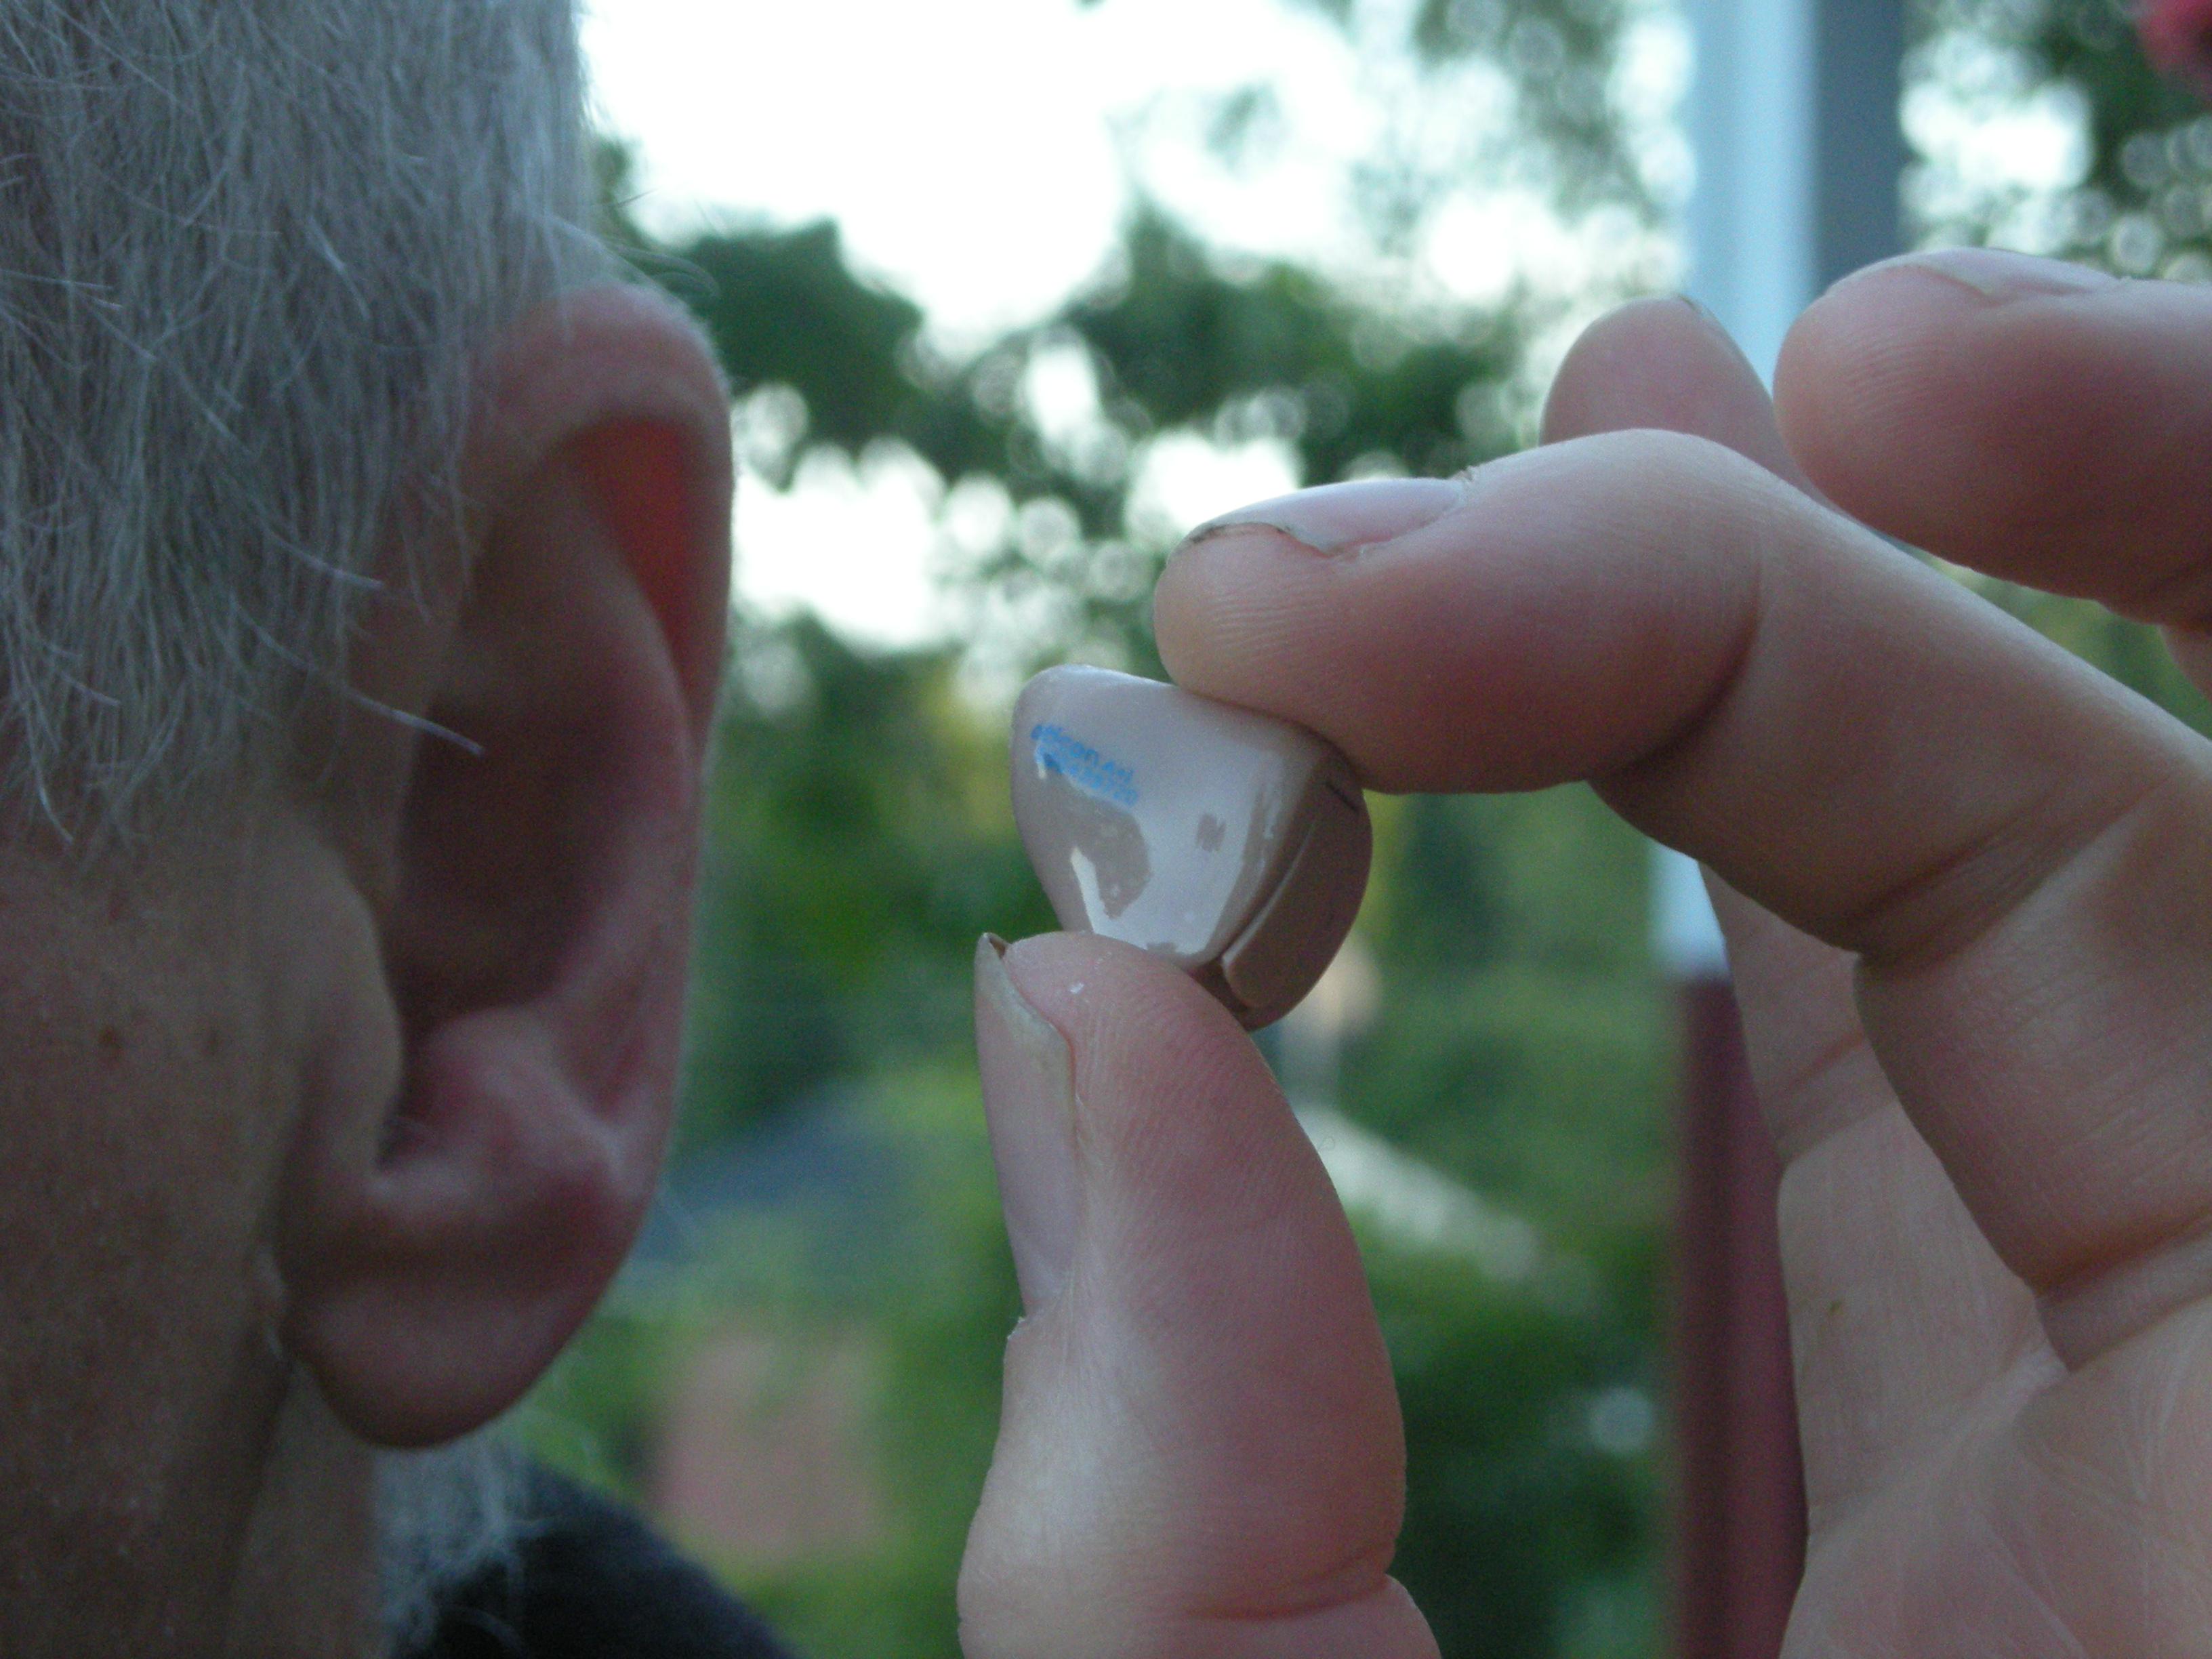
\includegraphics[width=\textwidth,height=0.7\textheight,keepaspectratio]{fig/Hearing_aid_20080620.jpg}
			}
			\caption{J. Bergsten (2008) \textit{Hearing Aid}. Wikimedia Commons}
			\end{figure}
		}
%		\only<2> {
%			\begin{figure}
%			\centering
%			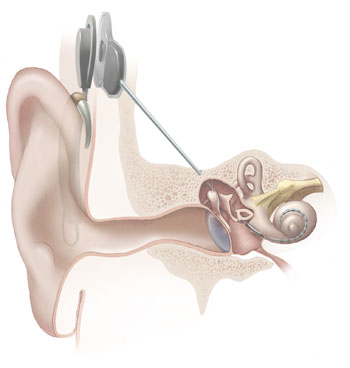
\includegraphics[width=\textwidth,height=0.55\textheight,keepaspectratio]{fig/Cochlear_implant.jpg}
%			\caption{United States Department of Health and Human Services (2005) \textit{Cochlear Implant}. Wikimedia Commons}
%			\end{figure}
%		}
		\only<2> {
			\begin{figure}
			\centering
			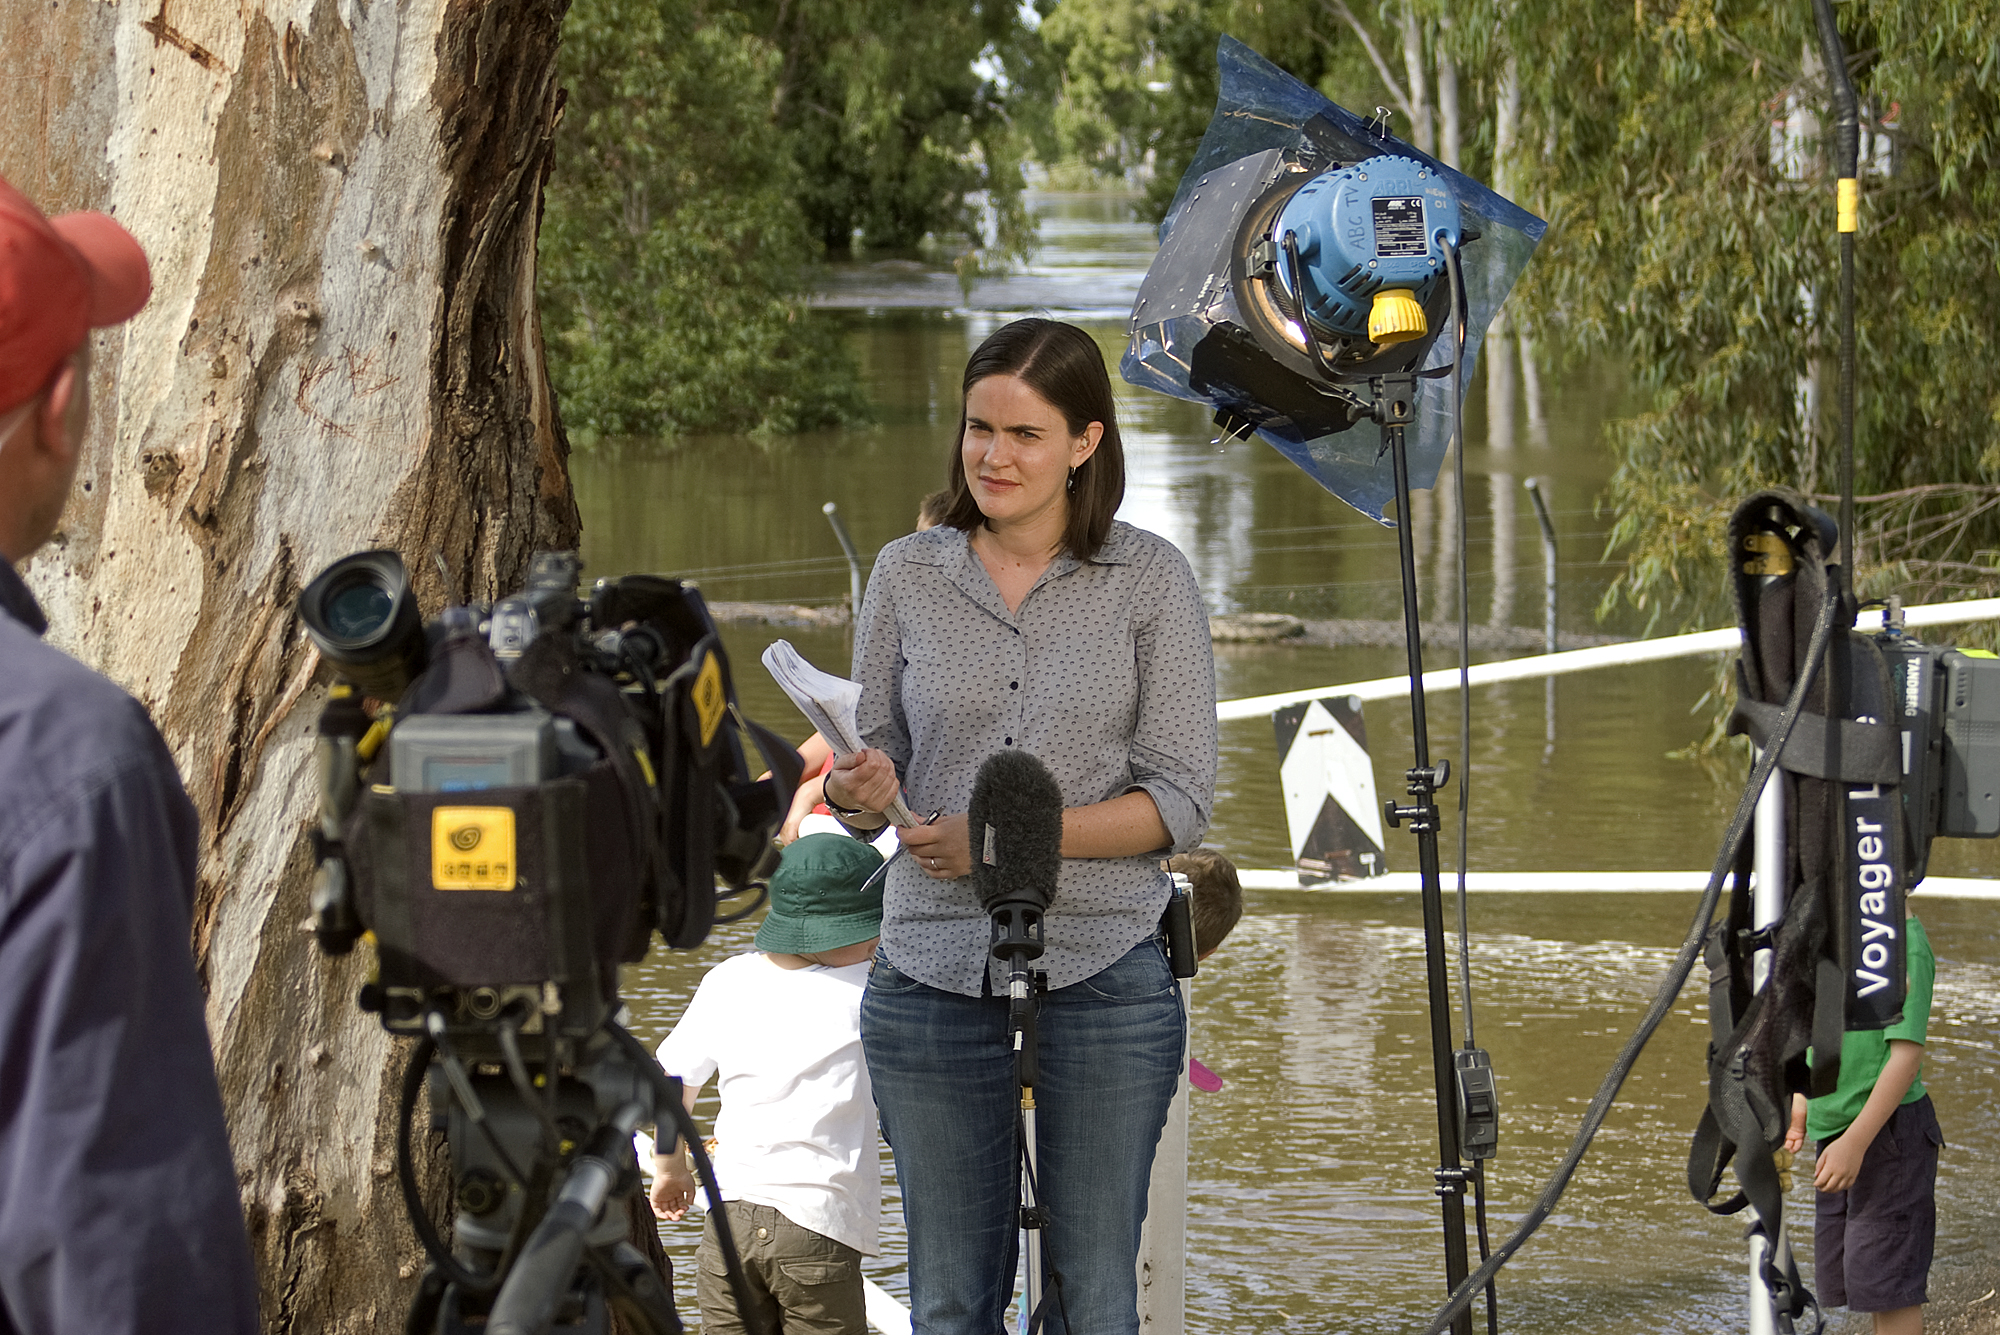
\includegraphics[width=\textwidth,height=0.7\textheight,keepaspectratio]{fig/ABC_News_reporter,_Naomi_Woodley,_waiting_to_do_a_live_report.jpg}
			\caption{Bidgee (2010) \textit{ABC News reporter, Naomi Woodley}. Wikimedia Commons}
			\end{figure}
		}
	\end{column}
	\begin{column}{0.45\textwidth}
		\begin{block}<1->{For Hearing Impaired}
			\begin{itemize}
				\small
				\item<1-> Hearing Aids
				\note<1>{Speech enhancement is, obviously, the process of enhancing speech.\par But why do we need to enhance speech? There are a number of applications.\par The greatest problem for the hearing impaired is hearing a voice where there are a number of competing voices around. This is known as babble noise.\par}
				\item<1-> Cochlear Implants
				\note<1>{Imagine a system where a hearing aid or cochlear implant user could train their device to recognise specific people they closely interact with. So a boy could set his cochlear implant to pick up only his mother's voice at the busy shopping center, or an elderly lady can tune her hearing aid into her husband's voice while at a busy cafe (bingo?).}
			\end{itemize}
		\end{block}
		\begin{block}<2->{For Telecommunications}
			\begin{itemize}
				\small
				\item Phone lines
				\note<2>{Speech enhancement is useful for the normal hearing population as well, for example over our mobile phone connections.\par Especially for use in extremely noisy environments.\par}
			\end{itemize}
		\end{block}
		\begin{block}<2->{For Recording}
			\begin{itemize}
				\small
				\item Cleaning sound in videos
				\note<2>{And not all speech enhancement cases require real-time processing. Speech enhancement can be used to improve the quality of prerecorded material as well.}
			\end{itemize}
		\end{block}
	\end{column}
	\end{columns}
\end{frame}
}
\begin{frame}{Why?}
	\begin{columns}[c]
	\begin{column}{0.5\textwidth}
		\only<1> {
			\begin{figure}
			\centering
			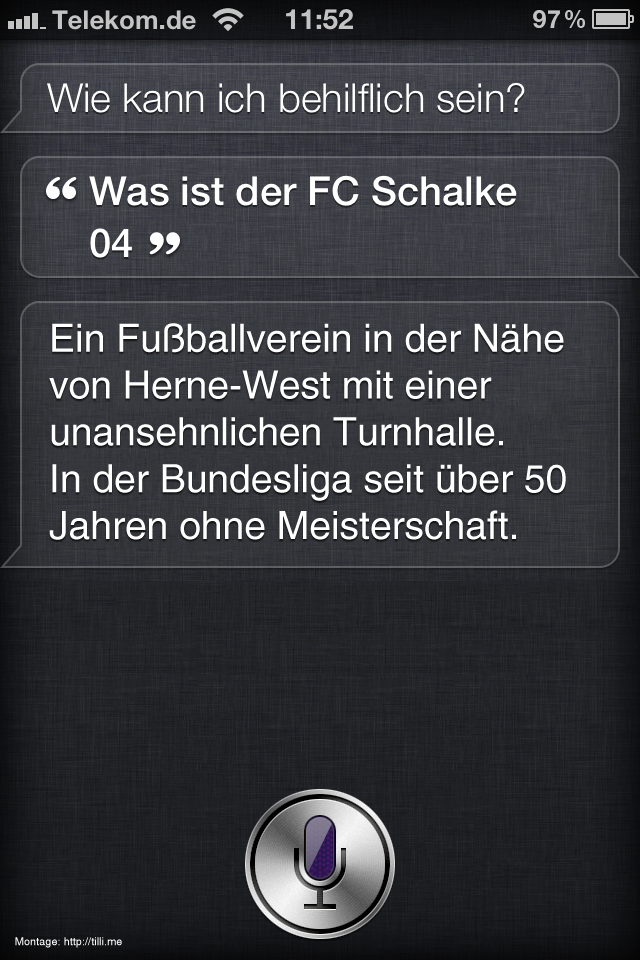
\includegraphics[width=\textwidth,height=0.65\textheight,keepaspectratio]{fig/Siri_German.png}
			\caption{H. Tillmann (2008) \textit{Fragt man Siri (iPhone 4S) nach dem FC Schalke 04}. Flickr}
			\end{figure}
			\note{The other side, then, are the applications for machines. Voice recognition has become much more popular in mobile phones. But anyone who has used these technologies before will know they aren't perfect, and should be used in a noise free environment.}
			%{https://www.flickr.com/photos/henningtillmann/6246291025/in/photolist-avXSGR-hygLb8-66a1zC-dPtqzW-fQjwAs-eSsC3H-hygHdp-aTLr7-7RgKY-azPRkn-6AeM92-8ywd2y-7E2DtG-8h9g9p-8sR7C8-qb8xC-8ygeYq-7cmKrL-p1sSPL-8tZAtV-4up52M-5ZtdN4-9iWWBk-6MvzVh-9PSefL-nHCmvx-8ygeYA-5ZxqBE-8YEp4-9PUDV3-bnkVy4-5A1EFv-di9TVx-gMhEGo-8Sq3ii-58Mqmy-d5agm-aKzpT4-dUm239-joZqKW-jp1aLA-7KRHqF-3b6w9n-aJuH3z-dNobZW-dsh41j-5jkQa1-8gUBxt-5ZtdQK-jRf19W}
		}
%		\only<2> {
%			\begin{figure}
%			\centering
%			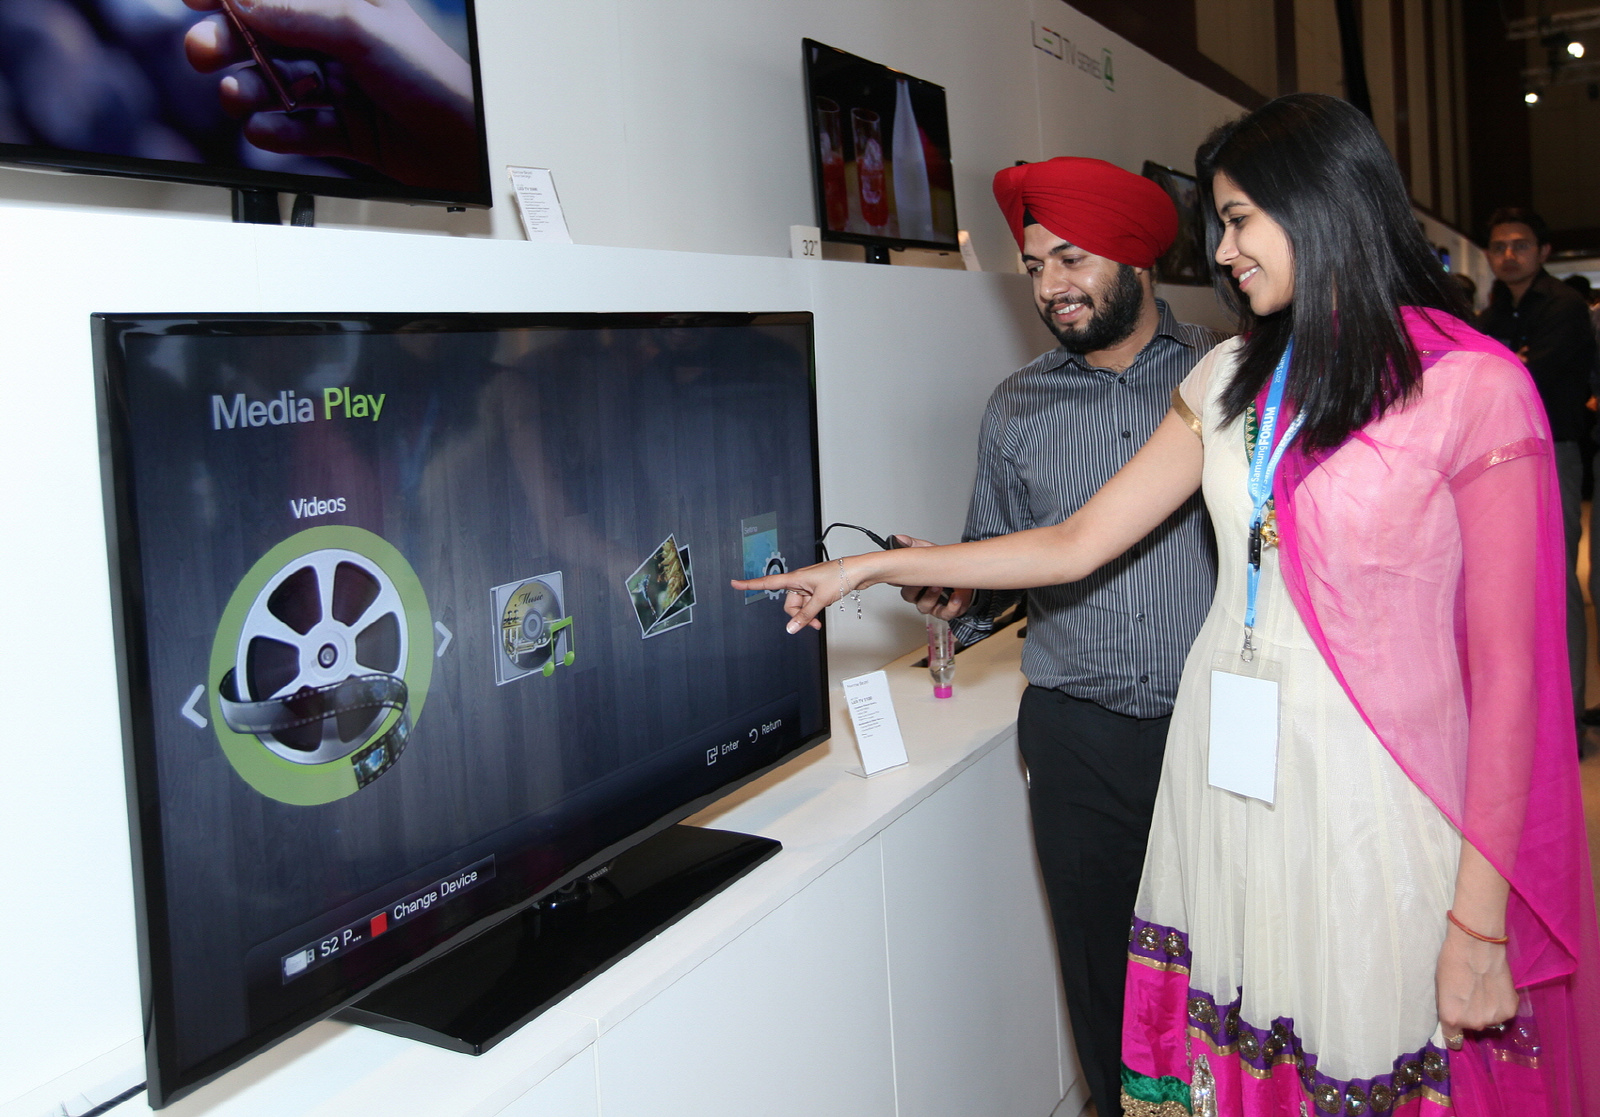
\includegraphics[width=\textwidth,height=0.6\textheight,keepaspectratio]{fig/Samsung_TV.jpg}
%			\caption{samsungtomorrow (2013) \textit{Samsung to Step up its Efforts to Enter Southwest Asia with Smart TV and Home Appliances}. Flickr}
%			\end{figure}
%			\note{The newest generation of televisions come with voice control features, as do many other consumer technologies.}
			%{https://www.flickr.com/photos/samsungtomorrow/8527481802/in/pool-1901913@N24/}
%		}
		\only<2> {
			\begin{figure}
			\centering
			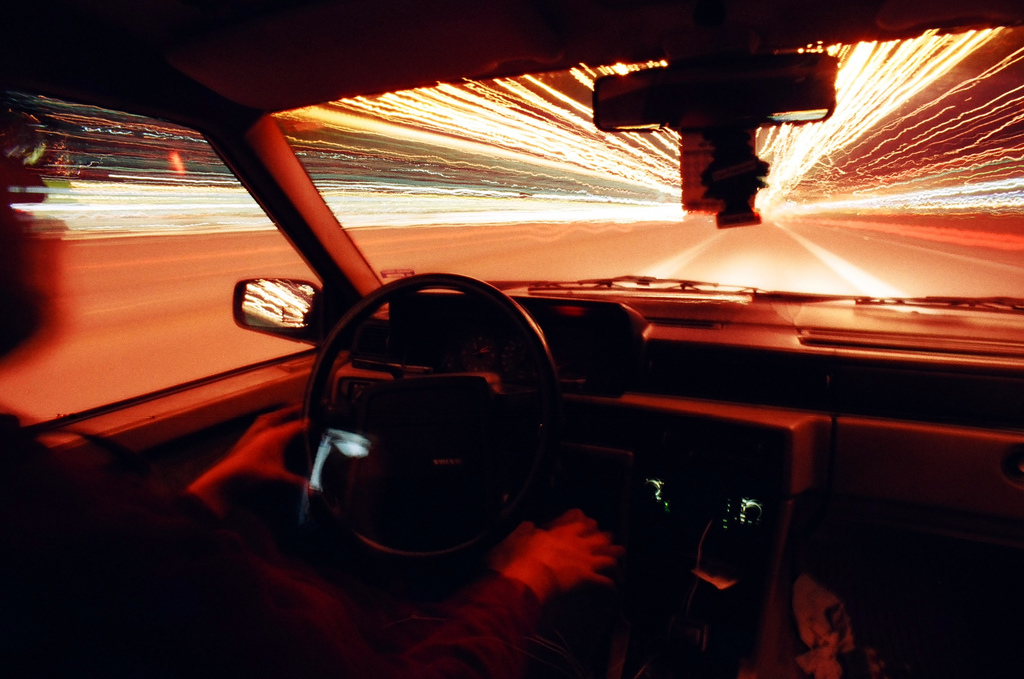
\includegraphics[width=\textwidth,height=0.6\textheight,keepaspectratio]{fig/driving.jpg}
			\caption{T. Anderson (2009) \textit{Driving the Volvo}. Flickr}
			\end{figure}
			\note{It can be important for humans to be able to interact with computers in non-traditional methods. This is called Human Computer Interaction, or HCI. For example, while driving, a computer cannot be safely interacted with in the usual way, but a voice control system is appropriate.}
		}
	\end{column}
	\begin{column}{0.4\textwidth}
		\begin{block}{For Machines}
			\begin{itemize}
				\item<1-> Mobile Phones
				\item<1-> Consumer Electronics
				\item<2-> To ease human-computer interaction
			\end{itemize}
		\end{block}
	\end{column}
	\end{columns}
\end{frame}
{\nologo
\begin{frame}{Two Applications}
	\framesubtitle{Human vs. Machine}
	\centering
	
\includegraphics[width=\textwidth,height=0.75\textheight,keepaspectratio]{fig/fight.png}
	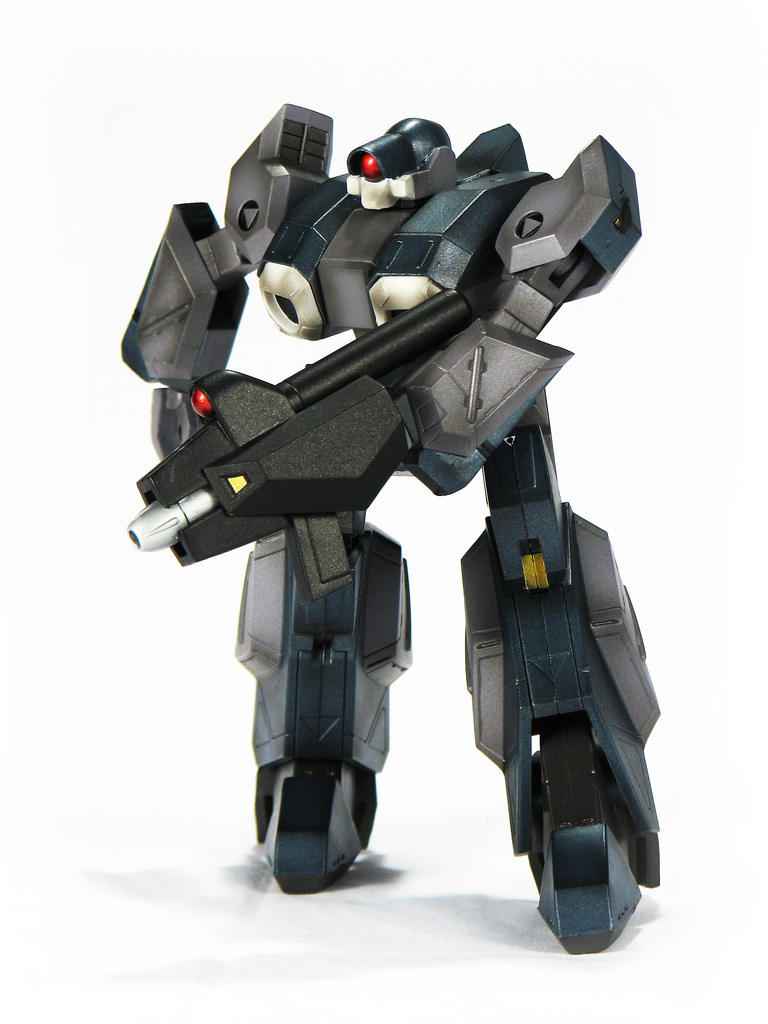
\includegraphics[width=\textwidth,height=0.75\textheight,keepaspectratio]{fig/robot.jpg}
	\note{So we can see many uses for speech enhancement, and that they generally fall into two categories, those for human and those for machines.}
\end{frame}
}

\subsection{Research Questions}
\begin{frame}{Research Questions}
	\begin{block}{Aims}
		\begin{itemize}
			\item To investigate and contrast evaluation measures for human listening and machine listening
			%\begin{itemize}
			%	\item Are human and machine listeners fundamentally different?
			%	\item Does an algorithm that provides enhancement for a human listener provide enhancement for a machine listener, and vice-versa?
			%\end{itemize}
			\item To develop phoneme-dependent modifications to Non-negative Matrix Factorisation (NMF) speech enhancement algorithms
		\end{itemize}
	\end{block}
	\note{My research aims were twofold. The first area sought to answer the question, if I have an algorithm that enhances speech for a human, will it be just as good for a machine? And vice versa.\par ---The second research aim was to then develop some modifications to existing algorithms, and to evaluate their performance using the methods found to be required in the first part.}
\end{frame}

\section{Human vs. Machine Evaluation}

\subsection{Intro}
{\nologo
\begin{frame}{Human vs. Machine Hearing}
	\begin{block}{How does a machine ``hear''?}
		\begin{itemize}
			\item Machine breaks the waveform into a relatively low number of features.
			\item Pattern recognition algorithms categorise based on these features.
		\end{itemize}
	\end{block}
	\begin{block}{How does a human ``hear''?}
		\begin{itemize}
			\item Humans hear from about 20Hz to 20kHz
			\item Humans listen to a lot more information, using the entire waveform
		\end{itemize}
	\end{block}
	\note{The reason we should consider human and machine enhancement separately is that the way humans and machines listen is fundamentally different. Machines break segments of a waveform down into a small number of features. It then uses these features to identify what is being spoken.\par However, a human listener listens to the entire waveform, over about 20Hz to 20kHz, which is a lot more information.\par So humans should be more sensitive to distortions in the signal.\par On the other hand, humans have an amazing brain to do some complex filtering, thereby enhancing speech on-the-fly.}
\end{frame}
}

%{\nologo
%\begin{frame}{Why does it matter?}
%	\hspace*{-9mm}
%	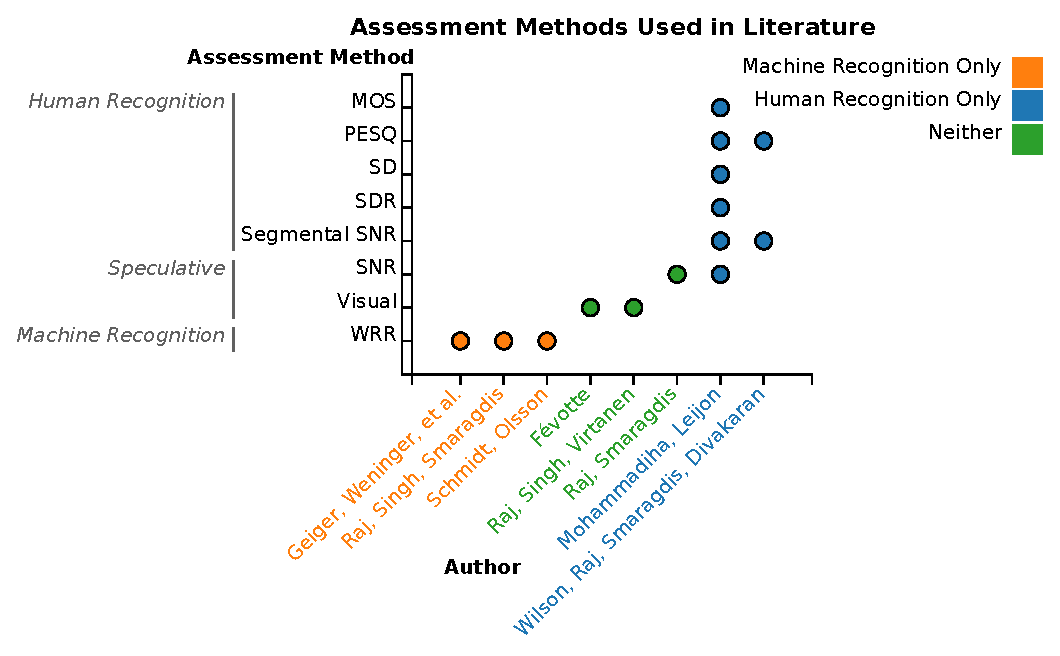
\includegraphics[width=\textwidth,height=0.9\textheight,keepaspectratio]{fig/assessmentMethods.eps}
%	\begin{textblock*}{0.3\paperwidth}(0.65\paperwidth,0.65\paperheight)
%	\begin{block}{Why?}
%	  Authors rarely measure both human and machine improvement.
%	\end{block}
%	\end{textblock*}
%	\note{As I looked into reports in literature, I noticed that when presenting novel enhancement algorithms, authors were very unlikely to consider enhancement and performance under different contexts.\par Here those highlighted in orange used only machine recognition methods, in this case the word recognition rate, and those highlighted in blue considered only human recognition. I will run through what MOS and PESQ mean shortly.\par What this means is that when I look through literature to decide which enhancement algorithm to use I am not getting the full picture, and can't be certain which algorithm is indeed the most appropriate.}
%\end{frame}
%}

\subsection{Methodology}
%\begin{frame}{Test Measures}
%	\begin{itemize}
%		\item MOS - Mean Opinion Score
%		\item PESQ - Perceptual Evaluation of Speech Quality
%		\item PRR - Phoneme Recognition Rate
%	\end{itemize}
%	\note{The test measures I considered were MOS, Mean Opinion Score, PESQ, Perceptual Evaluation of Speech Quality and PRR, Phoneme Recognition Rate.}
%\end{frame}
{\nologo
\begin{frame}{Test Measures}
	\begin{block}{MOS (Human)}
		Mean Opinion Score. Test subjects are asked to rate the perceived quality or speech.

		\begin{columns}[c]
		\begin{column}{0.4\textwidth}
			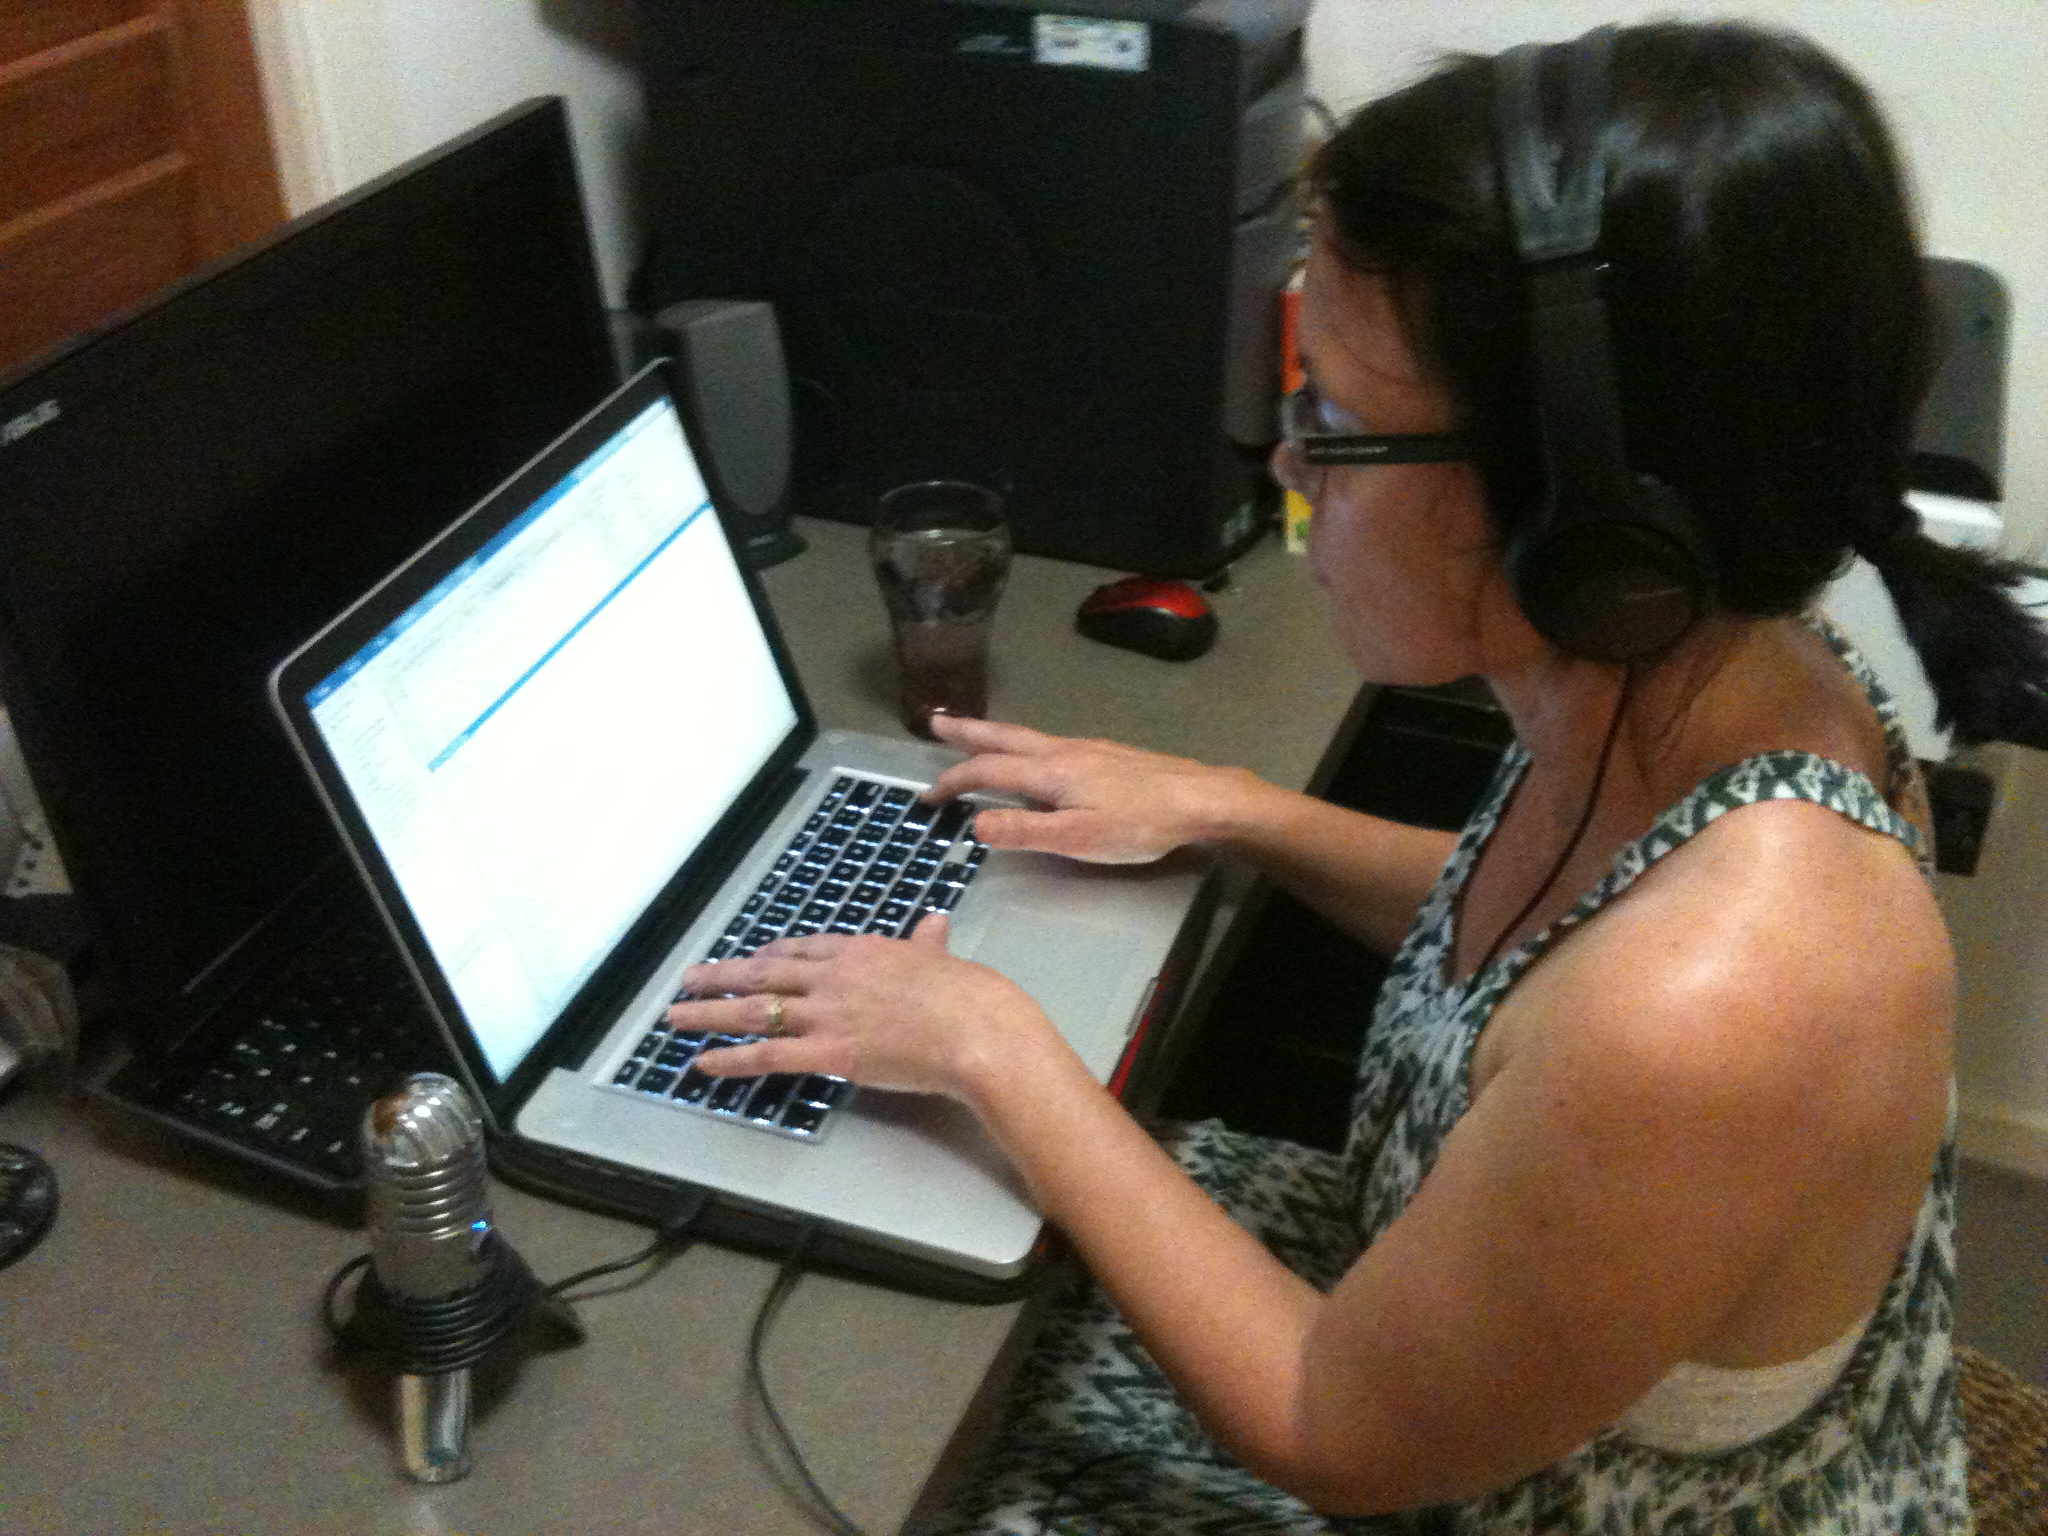
\includegraphics[width=\textwidth,height=0.8\textheight,keepaspectratio]{fig/mos.jpg}
		\end{column}
		\begin{column}{0.5\textwidth}
			\begin{tabular}{|c|c|}
			\hline 
			Quality of the speech & Score\tabularnewline
			\hline 
			\hline 
			Excellent & 5\tabularnewline
			\hline 
			Good & 4\tabularnewline
			\hline 
			Fair & 3\tabularnewline
			\hline 
			Poor & 2\tabularnewline
			\hline 
			Bad & 1\tabularnewline
			\hline 
			\end{tabular}
		\end{column}
		\end{columns}
	\end{block}
	\note{MOS is a subjective test, where human subjects are asked to listen to a number of recordings in a random order and rate their perceived quality. The score is then taken as the mean of the recorded scores.}
\end{frame}
}
\begin{frame}{Test Measures}
	\begin{block}{PESQ (Human)}
		Perceptual Evaluation of Speech Quality. MOS equivalent, but as an objective automated algorithm.
	\end{block}
	\begin{block}{PRR (Machine)}
		Phoneme Recognition Rate. Measure the phoneme recognition rate of an automated speech recognition system.
	\end{block}
	\note{PESQ is an algorithm that attempts to be equivalent to if a MOS test was completed. This is a lot quicker, easier, cheaper and gives an objective score. In general, the correlation with MOS scores has shown to be quite high when analysing telecommunication systems.\par The method I have used to measure machine recognition is the phoneme-level accuracy of an automated speech recognition system. I use the phoneme recognition as the phoneme is the building block of speech.}
\end{frame}
\begin{frame}{Phonemes}
	\large
	  \begin{spacing}{1.5}
		\begin{tabular}{r | l}
			Phrase & ``Examine a sentence.'' \\
			Words & ``Examine'' + ``a'' + ``sentence'' \\
			Syllables & /Ex.am.ine/ + /a/ + /sen.tence/ \\
			%Phonemes & (IH G Z AE M IH N) + (AH) + (S EH N T AH N S) \\
			Phonemes & \textipa{/I g z \ae{} m I n/ + /9/ + /s E n t 9 n s/} \\
		\end{tabular}
	\end{spacing}
	\note{If we split a sentence or phrase up, we get individual words. Splitting those words we get syllables. But splitting those down we get phonemes, the building blocks of speech.}
\end{frame}

\subsection{Results}
\begin{frame}{What does existing data indicate?}
	\hspace*{-9mm}
	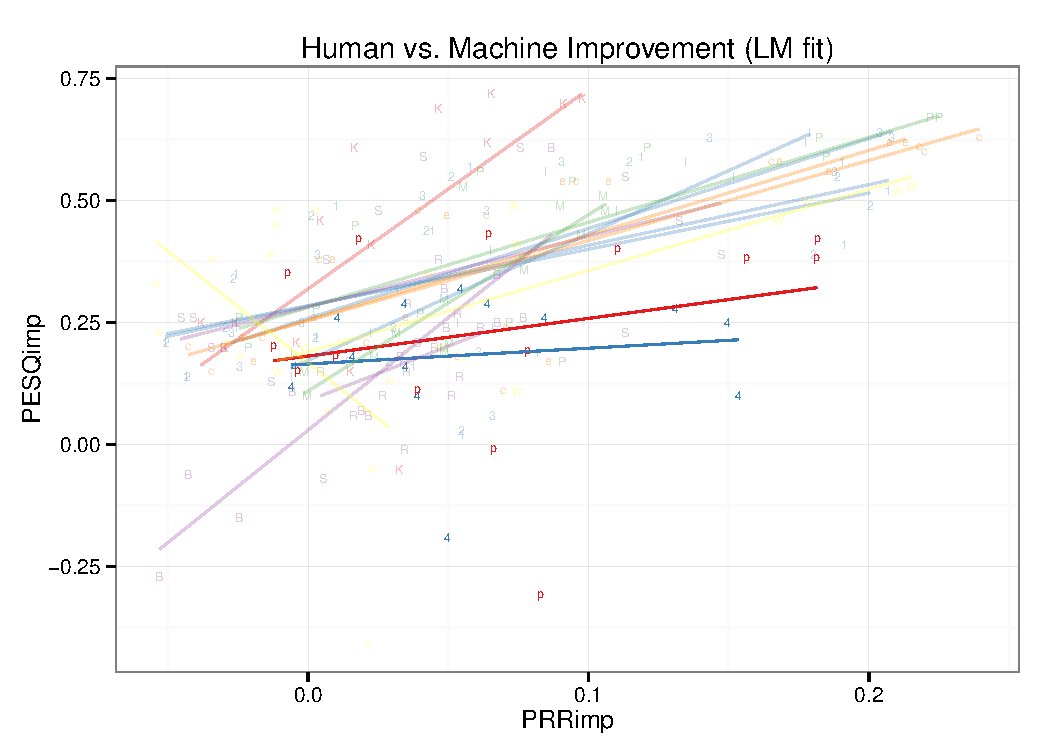
\includegraphics[width=0.6\paperwidth,height=0.8\textheight,keepaspectratio]{fig/HumanMachineAllLM.pdf}
	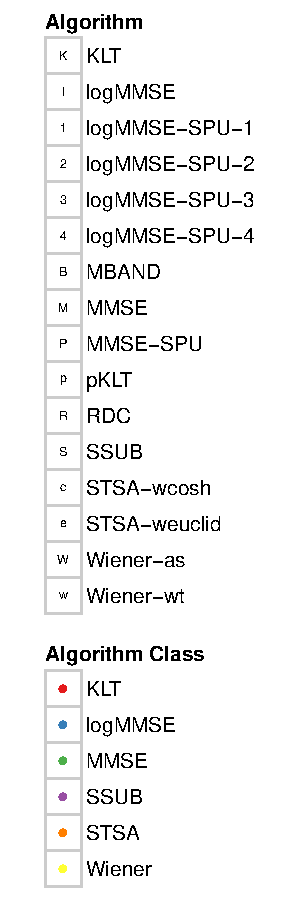
\includegraphics[width=0.4\paperwidth,height=0.65\textheight,keepaspectratio]{fig/HumanMachineAllLegend.pdf}
	\note{So I first conducted an investigation into some existing data, by pulling results from a number of different investigations and comparing similar algorithms under similar conditions.\par What we saw was in general, some correlation between the human and machine listeners.}
\end{frame}
\begin{frame}{What does existing data indicate?}
	\hspace*{-9mm}
	\includegraphics[width=0.6\paperwidth,height=0.8\textheight,keepaspectratio]{fig/HumanMachineAllLM1.pdf}
	\begin{textblock*}{0.3\paperwidth}(0.65\paperwidth,0.4\paperheight)
	\begin{block}{Algorithms B and K}
	  Similar machine performance. K performs much better for humans.
	\end{block}
	\end{textblock*}
	\note{There were some obvious exceptions, such as when algorithms B and K were contrasted. Here we saw these algorithms had similar enhancement performance for machines, but the K algorithm clearly performed much better for humans. In fact, it appears to have given some of the best enhancement of all the algorithms considered.}
\end{frame}
%\begin{frame}{What does existing data indicate?}
%	\hspace*{-9mm}
%	\includegraphics[width=0.6\paperwidth,height=0.8\textheight,keepaspectratio]{fig/HumanMachineAllLM2.pdf}
%	\begin{textblock*}{0.3\paperwidth}(0.65\paperwidth,0.4\paperheight)
%	\begin{block}{Why?}
%	  Authors rarely measure both human and machine improvement.
%	\end{exampleblock}
%	\end{textblock*}
%\end{frame}
%\begin{frame}{What does existing data indicate?}
%	\hspace*{-9mm}
%	\includegraphics[width=0.6\paperwidth,height=0.8\textheight,keepaspectratio]{fig/HumanMachineAllLM3.pdf}
%	\begin{textblock*}{0.3\paperwidth}(0.65\paperwidth,0.4\paperheight)
%	\begin{block}{Algorithms c, e and P}
%	  Displayed correlation between human and machine. Performed well for both.
%	\end{block}
%	\end{textblock*}
%	\note{Highlighted here are the best performing algorithms. We can see that for these well-performing algorithms the correlation is much higher.}
%\end{frame}
%{\nologo
%\begin{frame}{Human Results (My Tests)}
%	\only<1>{
%		\centering
%		\vspace*{-0.08\textheight}
%		\includegraphics[width=1.2\textwidth,height=0.99\textheight,keepaspectratio]{fig/CMOSbox1.pdf}
%	}
%	\only<2>{
%		\centering
%		\vspace*{-0.08\textheight}
%		\includegraphics[width=1.2\textwidth,height=0.99\textheight,keepaspectratio]{fig/CMOSbox2.pdf}
%	}
%\end{frame}
%\begin{frame}{Machine Results (My Tests)}
%	\only<1>{
%		\centering
%		\vspace*{-0.08\textheight}
%		\includegraphics[width=1.2\textwidth,height=0.99\textheight,keepaspectratio]{fig/PRRaccbox1.pdf}
%	}
%	\only<2>{
%		\centering
%		\vspace*{-0.08\textheight}
%		\includegraphics[width=1.2\textwidth,height=0.99\textheight,keepaspectratio]{fig/PRRaccbox2.pdf}
%	}
%\end{frame}
%}
%\begin{frame}{Human vs. Machine Results (My Tests)}
%	\centering
%	\includegraphics[width=\textwidth,height=0.8\textheight,keepaspectratio]{fig/cmos-prrcorrimp.pdf}
%	\raisebox{0.5\height}{
%		\includegraphics[width=0.2\textwidth,keepaspectratio]{fig/mos-prr-legV.pdf}
%	}
%	\note{So next I implemented a number of enhancement algorithms, and tested them using speech mixed with different types of noise.\par Here the the x-axis shows our machine improvement, the percentage of correctly identified phonemes, and the human measure on the y-axis is what's known as the comparative MOS result, so those above 0 were rated as an improvement, and those below 0 were distorted.\par We see here a significant correlation between the two measures.}
%\end{frame}
\begin{frame}{Human vs. Machine Results (My Tests)}
	\only<1> {
		\centering
		\includegraphics[width=\textwidth,height=0.85\textheight,keepaspectratio]{fig/cmos-prraccimp1.pdf}
		\hspace*{-10mm}
		\raisebox{0.5\height}{
			\includegraphics[width=0.2\textwidth,keepaspectratio]{fig/mos-prr-legV.pdf}
		}
	}
	\only<2> {
		\centering
		\includegraphics[width=\textwidth,height=0.85\textheight,keepaspectratio]{fig/cmos-prraccimp2.pdf}
		\hspace*{-10mm}
		\raisebox{0.5\height}{
			\includegraphics[width=0.2\textwidth,keepaspectratio]{fig/mos-prr-legV.pdf}
		}
	}
	\note{However, here we have changed the measure for machines to penalise false positives. This is important as false positives will cause problems when the machine then tries to recognise words and meaning. \par It can be seen that there is no longer correlation between the two.\par Noted here is the case of Wojcicki's Ideal binary mask algorithm's, seen in green and red in the lower right corner. These particular algorithms completely distorted recordings according to human listeners, however performed very well in the machine's accuracy improvement.}
\end{frame}

\subsection{Findings}
\begin{frame}{Research Question 1 Findings}
	Contrasting Human and Machine Enhancement
	\begin{block}{Findings}
		\begin{itemize}
			\item Very little correlation between human perception and accuracy of machine recogniser.
			\item The ideal binary mask improves accuracy of machine recogniser, however completely distorts the signal for a human listener.
		\end{itemize}
	\end{block}
	\note{So, in terms of contrasting enhancement for humans and machines, it looks like the correlation between improvement for humans and machines is quite insignificant.\par A specific example has been seen where a large improvement for machines is seen, however the same enhancement renders the signal unrecognisable to a human.}
\end{frame}

\section{Phoneme-Dependent NMF}

\subsection{Introduction}
\begin{frame}{Mohammadia's Algorithm}
	\begin{itemize}
		\item State-of-the-art Algorithm
		\item NMF based on Hidden Markov Models
		\item Ability to be trained for different noise types and adapt in real-time 
		\item Two algorithms, online and supervised.
	\end{itemize}
	\centering
	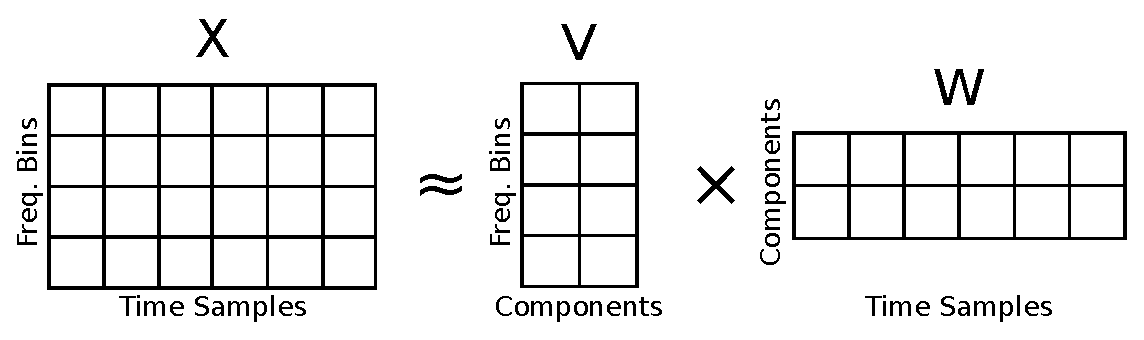
\includegraphics[width=\textwidth,height=0.25\textheight,keepaspectratio]{fig/NMF.eps}
	\note{I next looked at implementing an enhancement algorithm of my own. I decided to base the algorithm off a state-of-the-art NMF algorithm developed by Nasser Mohammadia.\par This algorithm used hidden markov models to model the noise, giving it the ability to be trained to different noise types and adapt in real time.}
\end{frame}
%{\nologo
%\begin{frame}{Phoneme-Dependent NMF}
%	\centerline{\includegraphics[height = 6cm]{fig/phoneme.png}}
%	{\tiny\begin{spacing}{0.5}
%		B. Raj, R. Singh, and T. Virtanen, ``Phoneme-Dependent NMF for Speech Enhancement in Monaural Mixtures,'' in INTERSPEECH, 2011, pp. 1217-1220.
%	\end{spacing}
%	}
%\end{frame}
%}

\subsection{Methodology}
\begin{frame}{Modified Training}
	\begin{columns}[c]
	\begin{column}{0.45\textwidth}
		\begin{block}{Drawn-Phoneme Training}
		Replacing the sentences provided for training with drawn phoneme slices.
		\end{block}
	\end{column}
	\begin{column}{0.55\textwidth}
		\hspace*{-7mm}
		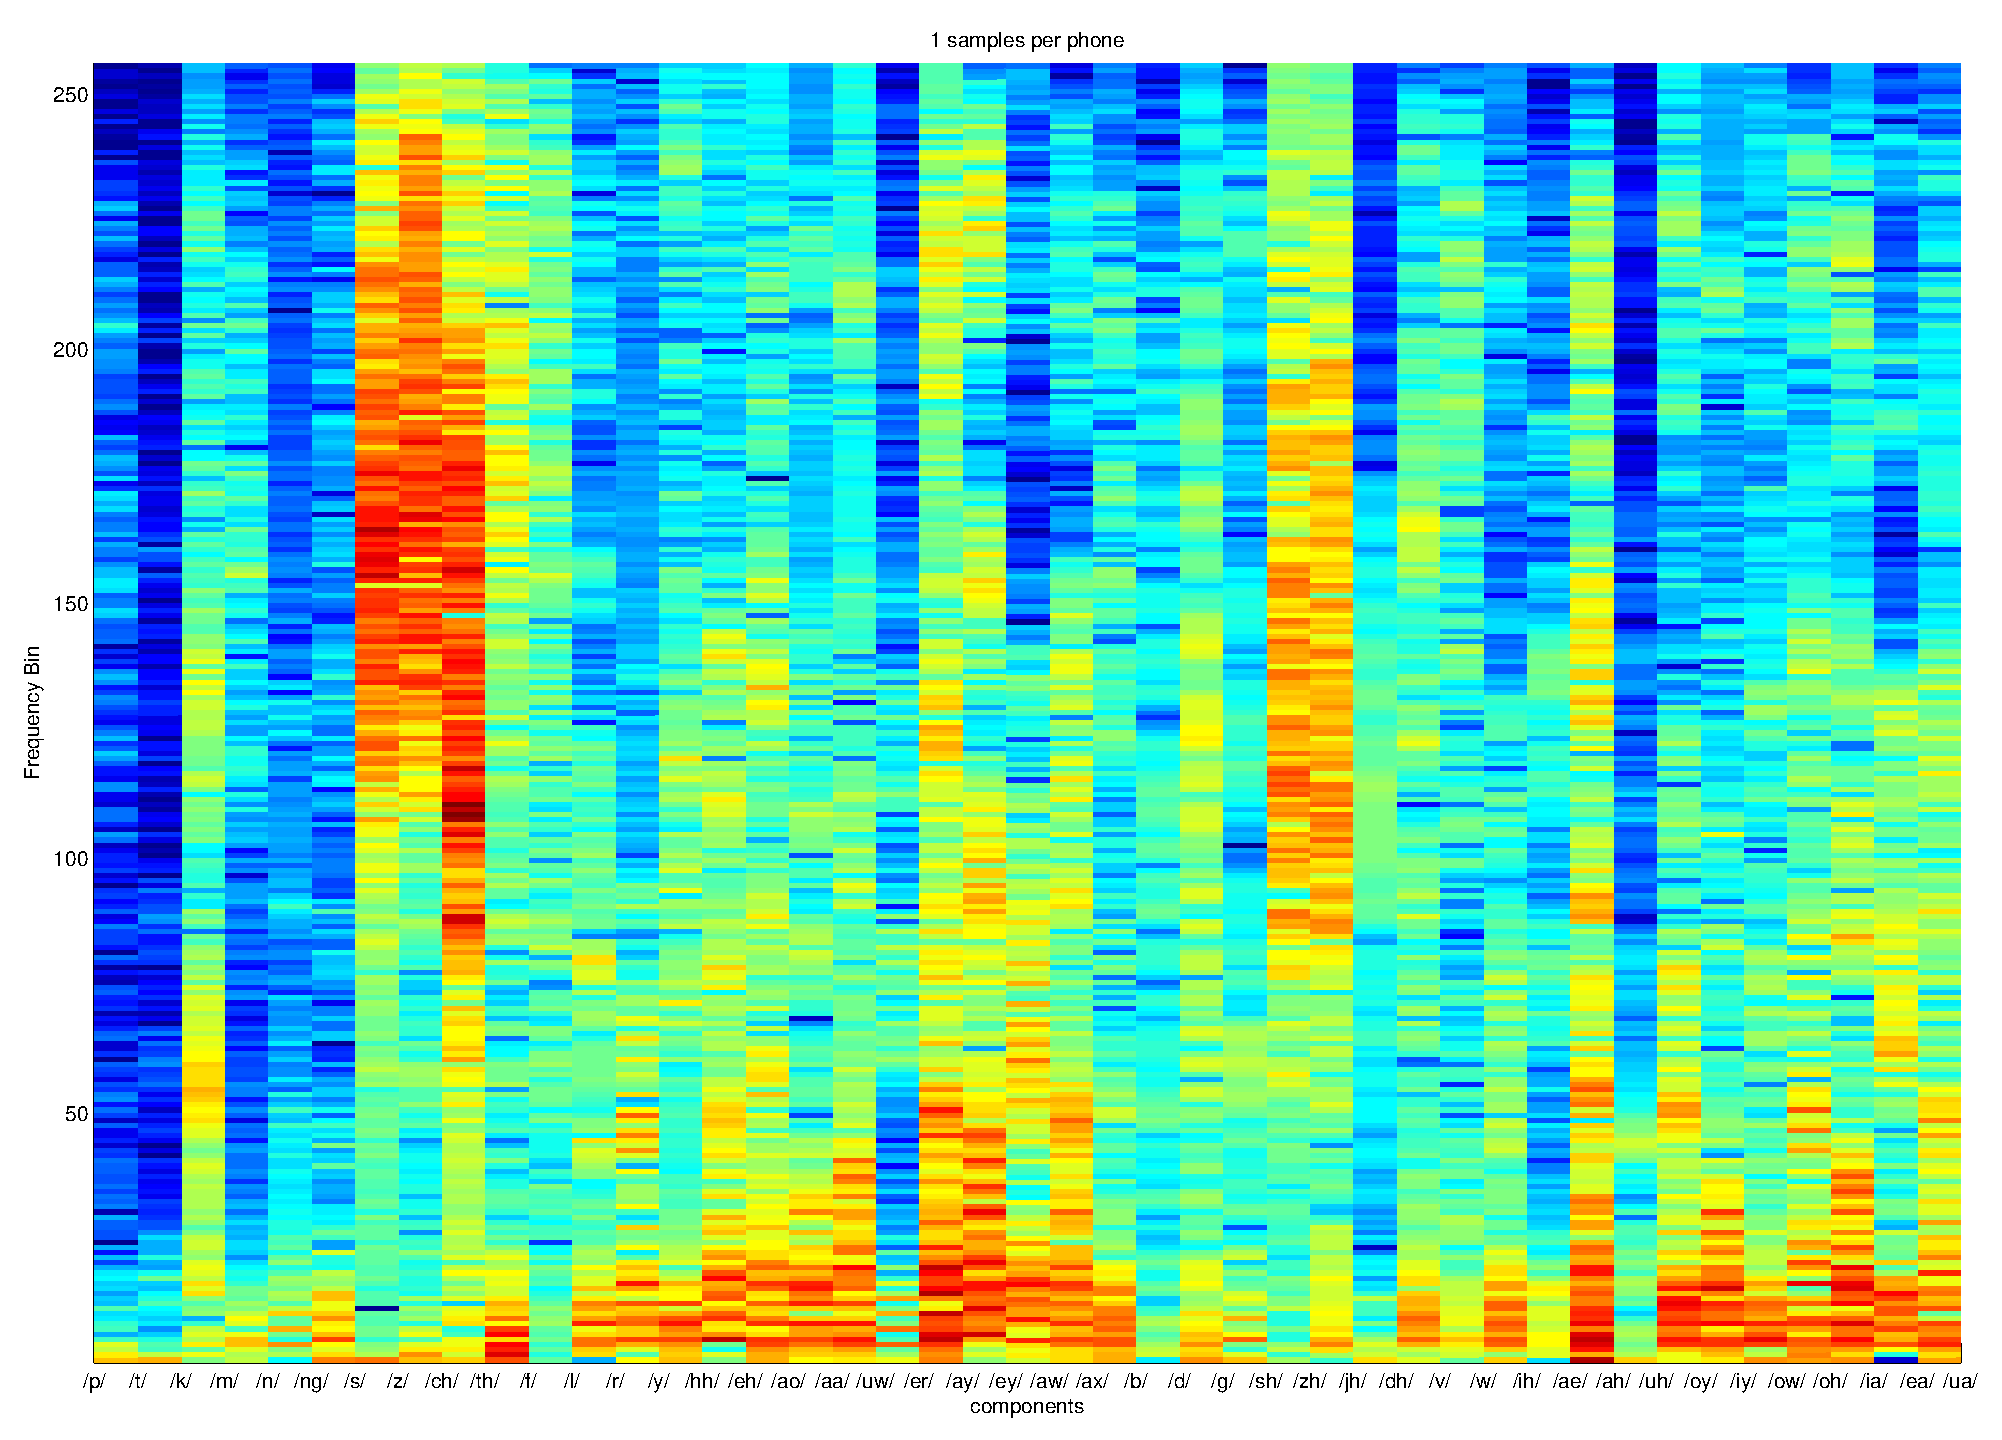
\includegraphics[width=1.15\textwidth,height=0.8\textheight,keepaspectratio]{fig/c3s-1phnSpectrogram.eps}
		\note{I have tested two methods of introducing this phoneme dependence. The first of these is instead of training the algorithm to the desired voice using recordings of sentences, to draw samples of each phoneme and using this as the training data.\par The idea was to provide higher density information to the training algorithm. The columns in the image here show the Fourier transform of the phoneme slices.}
	\end{column}
	\end{columns}
\end{frame}
%\begin{frame}{Modified Algorithm}
%	\begin{columns}[c]
%	\begin{column}{0.45\textwidth}
%		\begin{block}{Drawn-Phoneme Base}
%			\begin{itemize}
%				\item NMF algorithms have a dictionary they use to identify speech and extract it.
%				\item Here we will replace the dictionary with drawn phoneme slices.
%			\end{itemize}
%		\end{block}
%	\end{column}
%	\begin{column}{0.55\textwidth}
%		\hspace*{-7mm}
%		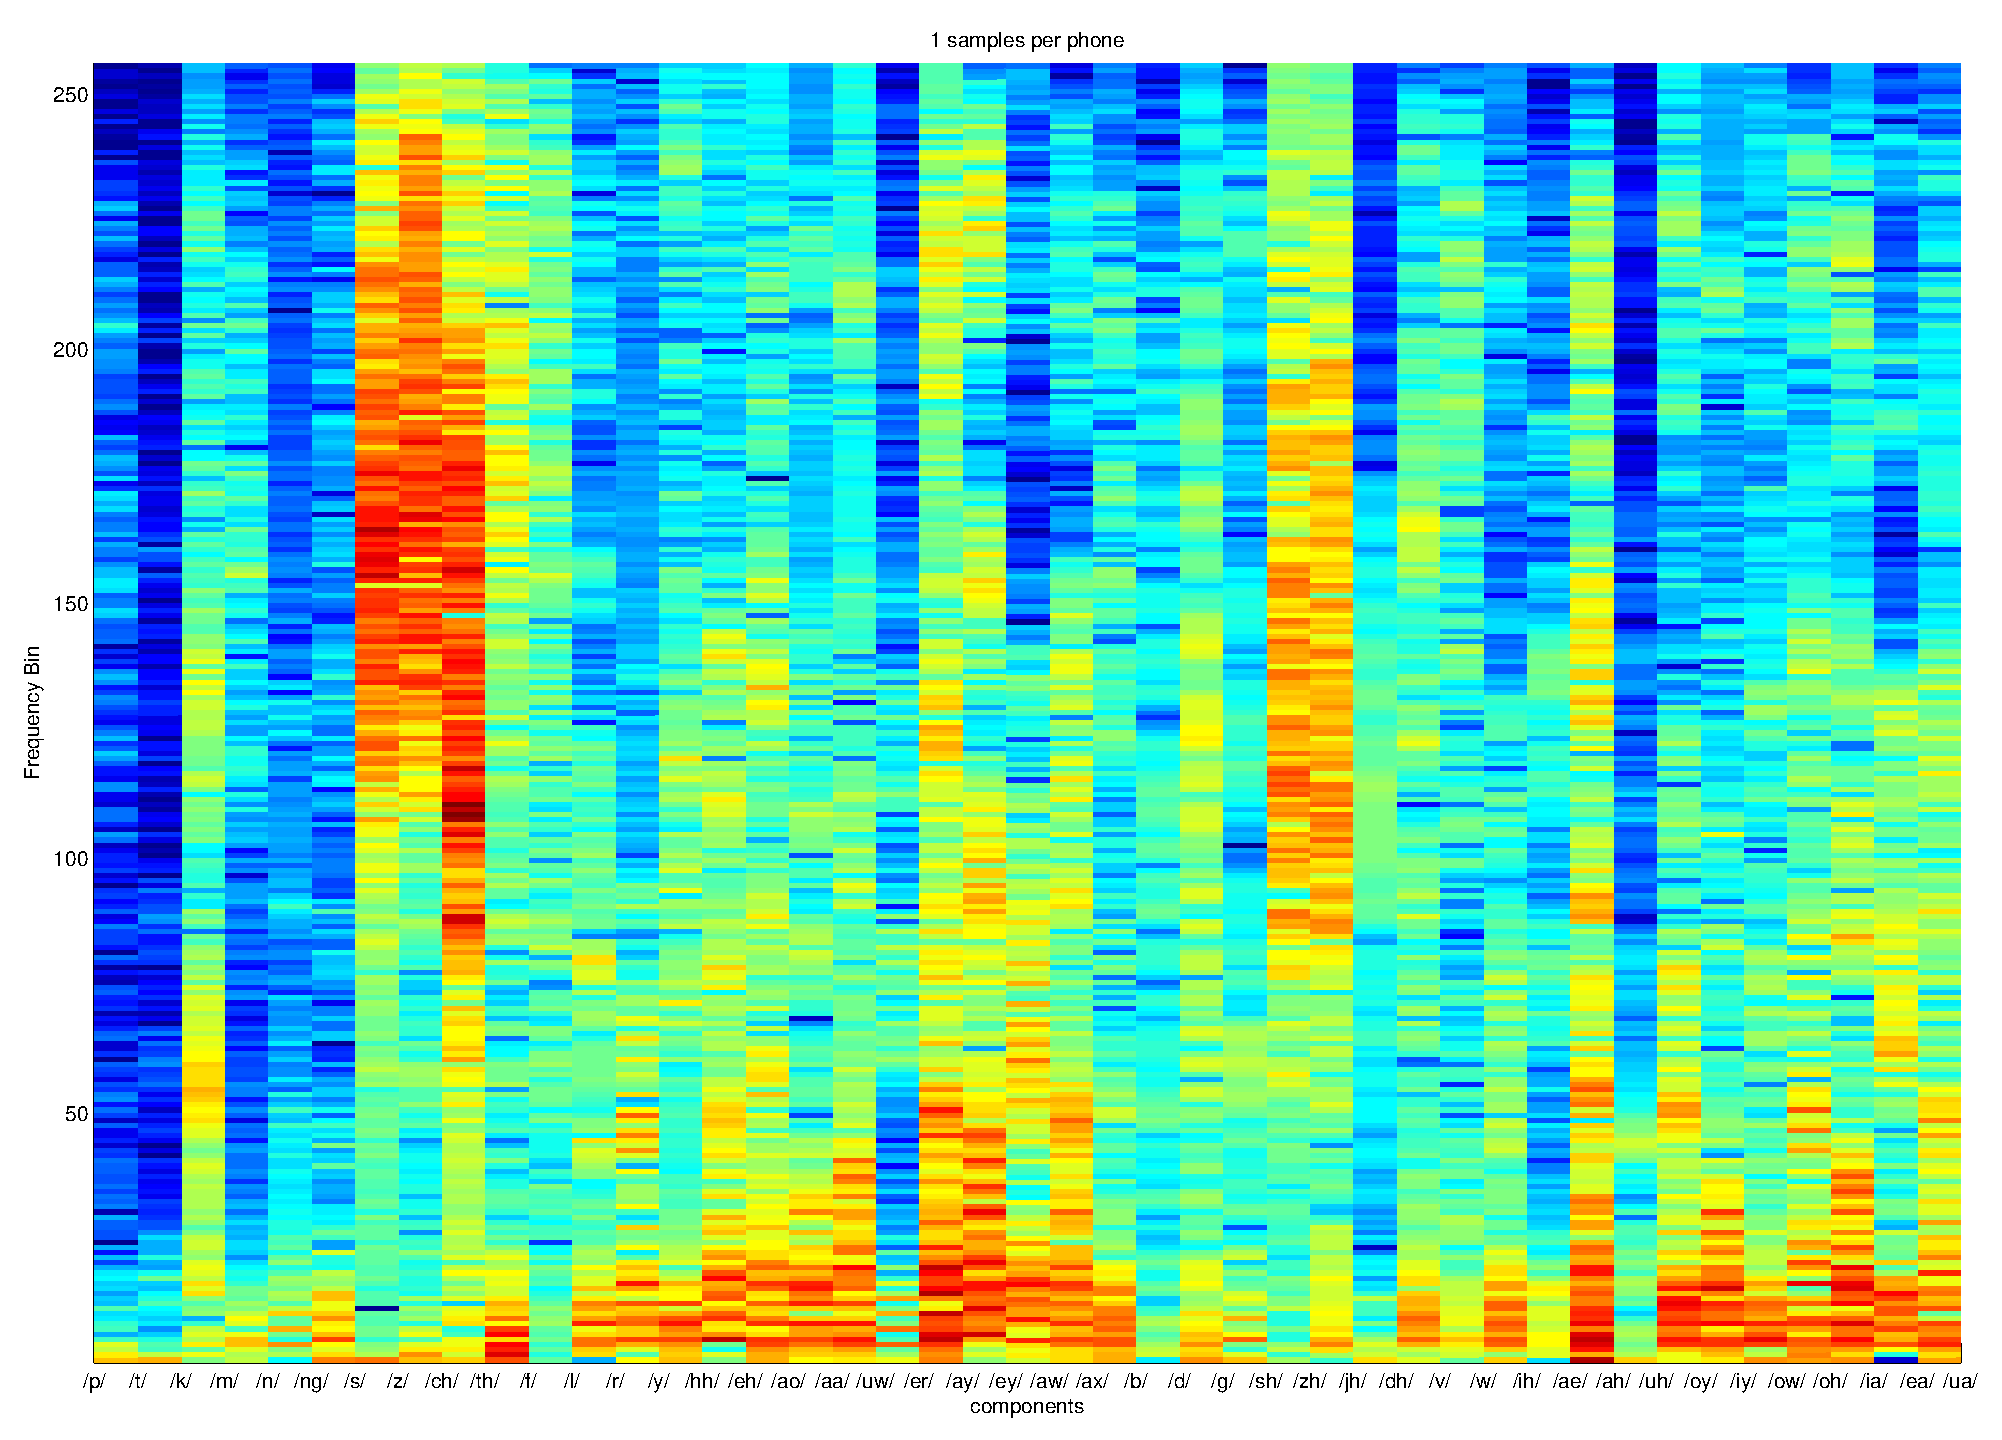
\includegraphics[width=1.15\textwidth,height=0.8\textheight,keepaspectratio]{fig/c3s-1phnSpectrogram.eps}
%		\note{The second proposed change bypasses the training all together. These NMF algorithms have a dictionary they use to identify speech and extract it. This modification replaces the dictionary with the drawn phoneme slices directly.}
%	\end{column}
%	\end{columns}
%\end{frame}

\subsection{Results}
{\nologo
\begin{frame}{Comparative MOS Accuracy Results}
	\vspace*{-5mm}
	\centering
	\includegraphics[height=0.9\textheight,keepaspectratio]{fig/CMOS_phnComp1.pdf}
	\note{Here are the comparative MOS results for each of my proposed methods, phoneme training and phoneme dictionary.\par Here the x-axis shows the original performance, and the y-axis shows the new performance. So those points below the line were worse, and those above the line were improved.
As we can see, some points are better, some points are worse, but overall there is no significant trend of improvement for the human listeners.}
\end{frame}
\begin{frame}{PRR Accuracy Results}
	\only<1>{
		\vspace*{-5mm}
		\centering
		\includegraphics[height=0.9\textheight,keepaspectratio]{fig/PRRaccImp_phnComp1.pdf}
		\note{Here we have the same results, but for a machine recogniser.
Here we see something interesting: in general, the phoneme training, on the left, does indeed improve the results.}
	}
	\only<2>{
		\vspace*{-5mm}
		\centering
		\includegraphics[height=0.9\textheight,keepaspectratio]{fig/PRRaccImp_phnComp2.pdf}
		\note{Especially note the car noise tests, indicated by the plus signs, which previously were negative or distorting, but are now positive, so enhanced.}
	}
%	\only<3>{
%		\vspace*{-5mm}
%		\centering
%		\includegraphics[height=0.9\textheight,keepaspectratio]{fig/PRRaccImp_phnComp3.pdf}
%		\note{However, we can see that phoneme training performs much more poorly when the noise was a single competing speaker of the same sex, indicated by the circles.}
%	}
%	\only<4>{
%		\vspace*{-20mm}
%		\hspace*{-15mm}
%		\includegraphics[width=1.3\textwidth,keepaspectratio]{fig/PRRaccImp_phnComp4.pdf}
%		\note{We can also see that the phoneme dictionary modification seems to squeeze all the results into a smaller vertical area. This modification improves the previously poor performers, but distorts the good performers.}
%	}
\end{frame}
}

\section{Conclusion}

\subsection{Research Question 1}
\begin{frame}{Research Question 1 Conclusions}
	\begin{block}{Recommended Measures}
		\begin{itemize}
			\item PESQ
			\item MOS, using a small population
			\item Word recognition rate of machine
		\end{itemize}
	\end{block}
	\note{Therefore, it is recommended that in future, authors proposing novel enhancement algorithms should use both human measures, in the form of PESQ, and where possible, MOS also. Even if this is only conducted on a small test sample. And the algorithm should also be tested for improvement for machine recognisers.}
\end{frame}
\begin{frame}{What does this mean?}
	\fontsize{5cm}{1em}\rmfamily\centering ``Context''
	\note{It is important to note the importance of context and considering the application.\par Had I have implemented my algorithm and only tested the enhancement for human listeners I may never have seen the potential of these phoneme-dependent algorithms.\par Conversely, had I have tested them only against machines, others may have used my algorithms and wasted a lot of time trying to use them for human speech enhancement.}
\end{frame}

\subsection{Research Question 2}
\begin{frame}{Research Question 2 Conclusions}
	Phoneme-Dependence for NMF Algorithms
	\begin{block}{Conclusions}
		\begin{itemize}
			\item Phoneme training generally improves algorithm for machine recognisers
			\begin{itemize}
				\item Although not where noise is very similar to voice, such as same sex competing speaker
			\end{itemize}
			\item No significant improvements for human listeners
		\end{itemize}
	\end{block}
	\note{So we can conclude that using phoneme training in general gives better enhancement for machines. The exception was where our noise is extremely similar to the voice, in which case we have a poorer performance.\par We also saw that using the phoneme dictionary improved some of the previously bad performing results. This could be exploited by a smart algorithm that knows which enhancement algorithm to use depending on the context.\par We noted no significant improvements for humans.}
\end{frame}
{\nologo\usebackgroundtemplate{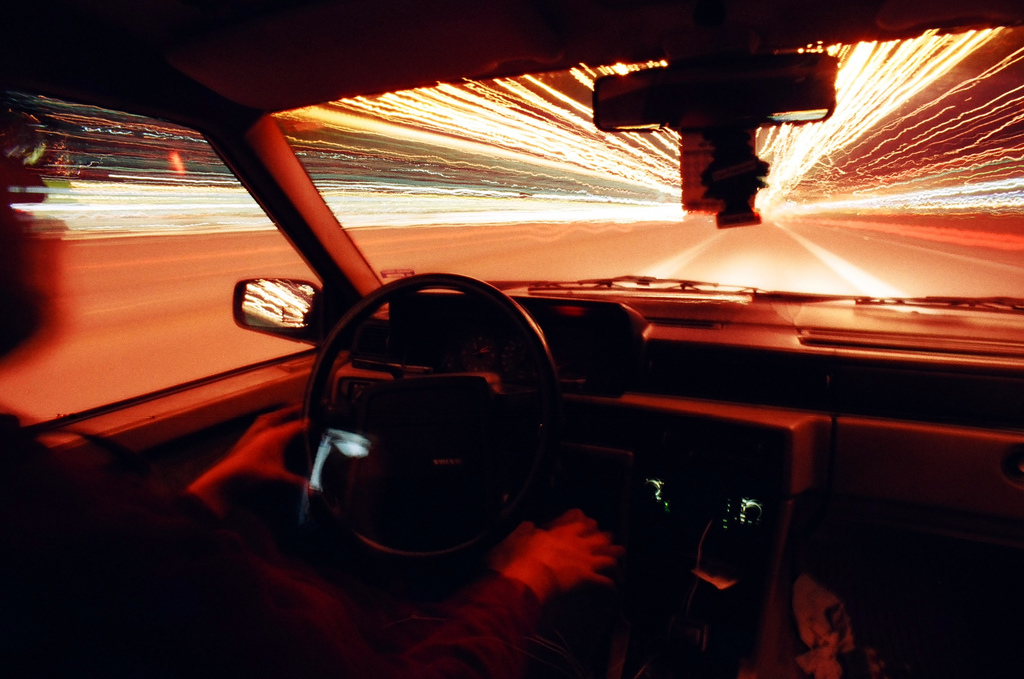
\includegraphics[width=\paperwidth]{fig/driving.jpg}}%
\begin{frame}{What does this mean?}
	\note{The phoneme dependent algorithms I have created performed very well against noise recordings from within a car. So such algorithms could easily find application for in-car electronics such as car radios, GPS systems and hands-free systems.}
\end{frame}
}
%\begin{frame}{Further Studies}{Where to from here?}
%	\begin{block}{}
%		\begin{itemize}
%			\item Investigate machine word recognition rate
%			\item Noise context dependent enhancement
%		\end{itemize}
%	\end{block}
%	\note{In terms of future work, there are a number of investigations that could stem from this work.\par Similar studies to mine could be conducted using the machine word recognition rate, which would give further insight into the machine's ability to recognise meaning.\par And investigations could be done into using different enhancement algorithms depending on the type of noise present to get the most efficient enhancement, rather than a one size fits all approach.}
%\end{frame}

{
\usebackgroundtemplate{\includegraphics[width=\paperwidth]{poster.pdf}}%
\frame[plain]{}
}

\appendix
\newcounter{finalframe}
\setcounter{finalframe}{\value{framenumber}}


{\nologo
\begin{frame}
	\centering
	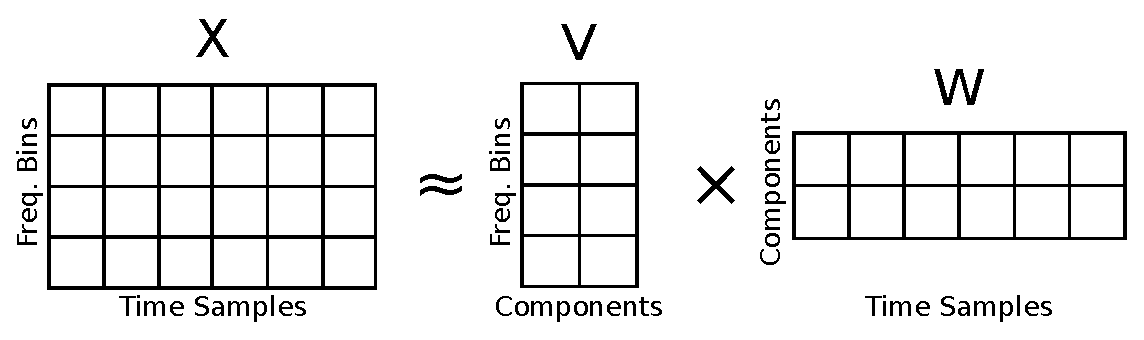
\includegraphics[width=\textwidth,height=0.9\textheight,keepaspectratio]{fig/NMF.eps}
\end{frame}
\begin{frame}
	\centering
	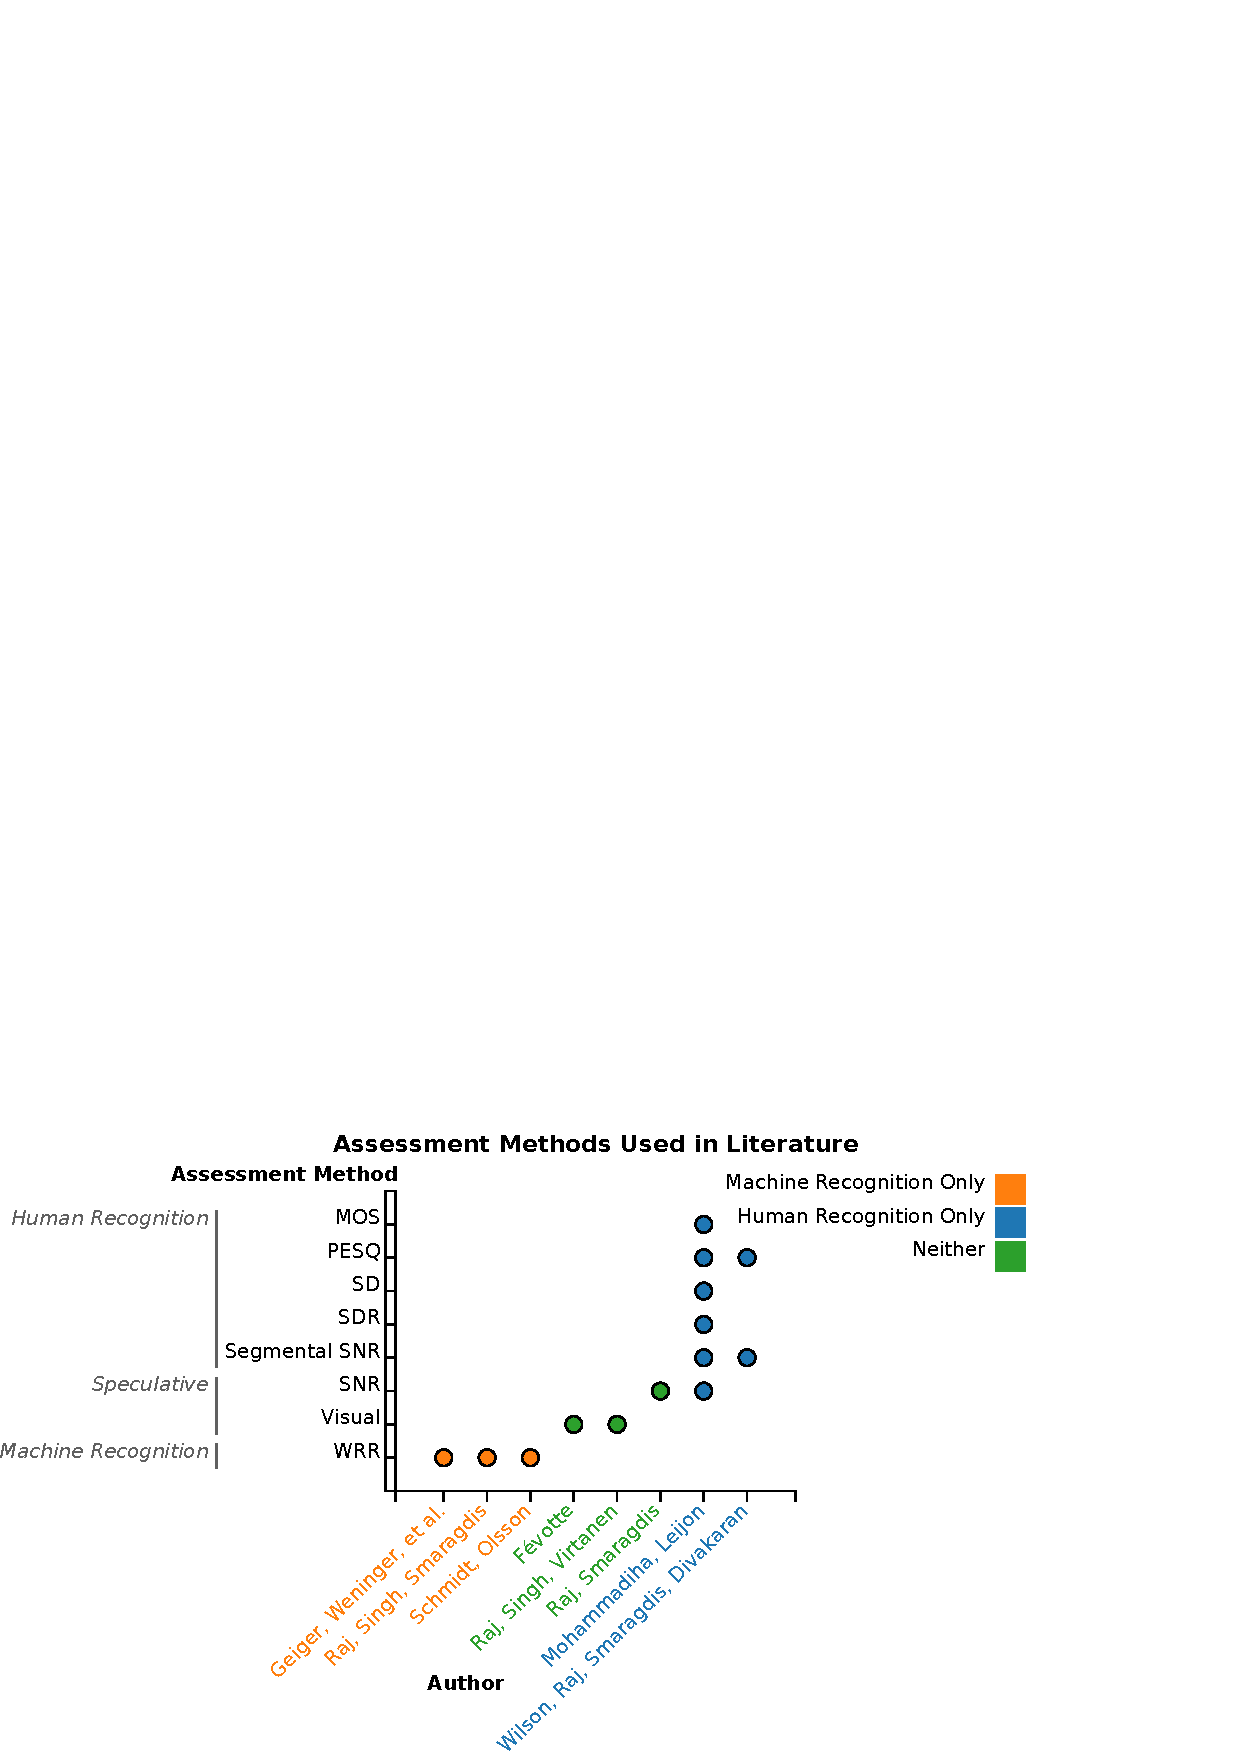
\includegraphics[width=\textwidth,height=0.9\textheight,keepaspectratio]{fig/assessmentMethods.pdf}
\end{frame}
}

\setcounter{framenumber}{\value{finalframe}}

\end{document}